\documentclass[tikz,border=8pt]{standalone}
% Shared look for every TikZ diagram. Load with \input{../../tools/tikz-style.tex}
\usepackage[T1]{fontenc}
\usepackage{lmodern}
\renewcommand{\sfdefault}{lmr}  % diagrams use the same serif as the text
\usetikzlibrary{arrows.meta, positioning, shapes.geometric, calc, fit, backgrounds}
\definecolor{cblue}{HTML}{4C78A8}
\definecolor{corange}{HTML}{F58518}
\definecolor{cgreen}{HTML}{54A24B}
\definecolor{cred}{HTML}{E45756}
\definecolor{cpurple}{HTML}{B279A2}
\definecolor{cgrey}{HTML}{6B6B6B}
\tikzset{
  every picture/.style={font=\sffamily, line width=1.2pt},
  box/.style={draw=#1, fill=#1!12, rounded corners=4pt, align=center, inner sep=7pt, minimum height=1.1cm},
  box/.default=cgrey,
  arrow/.style={-{Stealth[length=3mm]}, draw=cgrey, line width=1.4pt},
  title/.style={font=\sffamily\bfseries\Large},
  note/.style={font=\sffamily\small, text=cgrey, align=center},
}
\AtBeginDocument{\hyphenpenalty=10000 \exhyphenpenalty=10000}

% Pose of a floor robot: world frame, robot at (2, 1) facing 30 degrees, body frame x_b (forward) and y_b (left).
\begin{document}
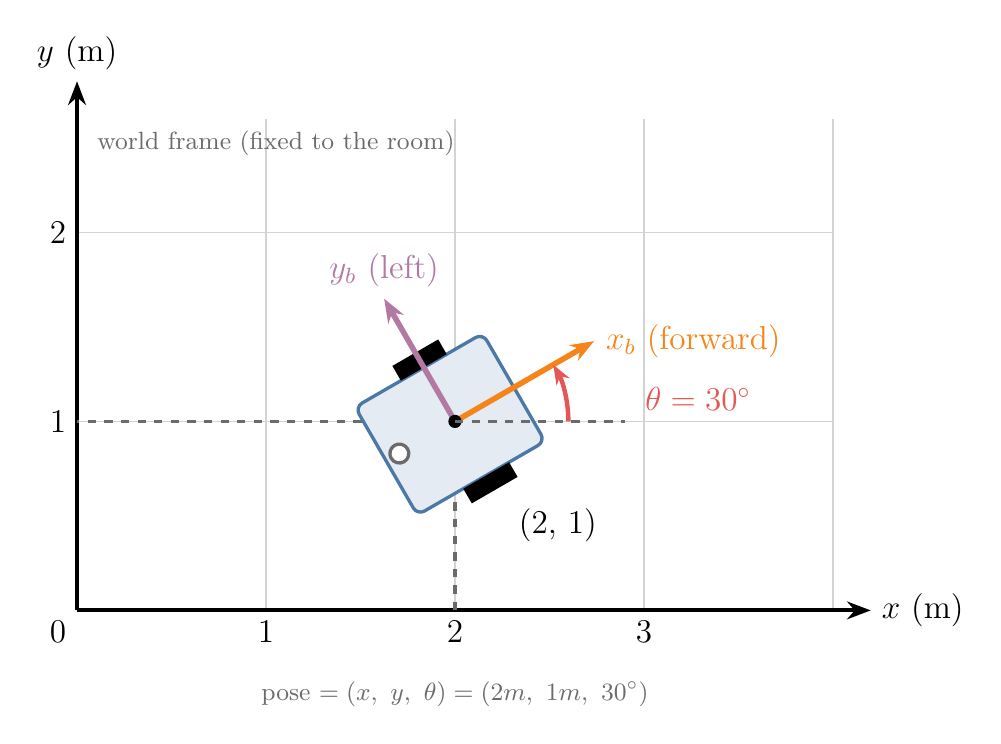
\begin{tikzpicture}[scale=2.4, every node/.append style={font=\large}]
  \draw[cgrey!30, line width=0.6pt] (0,0) grid (4,2.6);
  \draw[arrow, draw=black] (0,0) -- (4.2,0) node[right] {$x$ (m)};
  \draw[arrow, draw=black] (0,0) -- (0,2.8) node[above] {$y$ (m)};
  \foreach \i in {1,2,3} \node[below] at (\i,0) {\i};
  \foreach \i in {1,2} \node[left] at (0,\i) {\i};
  \node[below left] at (0,0) {0};
  \node[note, anchor=south west] at (0.05,2.35) {world frame (fixed to the room)};
  \draw[dashed, cgrey] (2,0) -- (2,1) -- (0,1);
  \begin{scope}[shift={(2,1)}, rotate=30]
    \draw[cblue, fill=cblue!15, rounded corners=3pt] (-0.42,-0.33) rectangle (0.36,0.33);
    \fill[black] (-0.14,0.33) rectangle (0.14,0.42);
    \fill[black] (-0.14,-0.42) rectangle (0.14,-0.33);
    \draw[cgrey, fill=white] (-0.34,0) circle (0.05);
    \draw[-{Stealth[length=3mm]}, corange, line width=2pt] (0,0) -- (0.85,0) node[right] {$x_b$ (forward)};
    \draw[-{Stealth[length=3mm]}, cpurple, line width=2pt] (0,0) -- (0,0.75) node[above] {$y_b$ (left)};
  \end{scope}
  \fill[black] (2,1) circle (0.035);
  \draw[cgrey, dashed] (2,1) -- (2.9,1);
  \draw[cred, line width=1.6pt, -{Stealth[length=2.5mm]}] (2.6,1) arc (0:30:0.6);
  \node[cred, right] at (2.95,1.12) {$\theta = 30^\circ$};
  \node[right, fill=white, inner sep=2pt] at (2.3,0.45) {$(2,\,1)$};
  \node[note, anchor=north] at (2,-0.32) {pose $= (x,\ y,\ \theta) = (2\text{ m},\ 1\text{ m},\ 30^\circ)$};
\end{tikzpicture}
\end{document}
